\chapter{Szum pomiarowy}
Szum pomiarowy występuje praktycznie przy każdym rodzaju pomiarów fizycznych i wynika on z wielu czynników np. niedokładność urządzenia pomiarowego. Aby sprawdzić odporność działania regulatora na taki właśnie szum pomiarowy posłużyliśmy się białym szumem guasowaskim. Jest to taki szum którego widmo jest płaskie, tzn. występują w nim wszystkie częstotliwości w równym natężeniu.
\subsection{Realizacja w Matlabie}
W celu wygenerowania białego szumu posłużyliśmy się funkcją \verb|wgn(m,n,power)|, która generuje $m$ próbek białego gaussowskiego szumu dla $n$ kanałów o podanej mocy w \verb|dBW|. Po wygenerowaniu takiej próbki, była ona dodawana do wartości zakłócenia używanej w regulacji (nie była ona natomiast dodawana do wartości zakłócenia podawanej do obiektu). \\
Jako zakłócenie bazowe zostało wykorzystane zakłócenie zmienne sinusoidalnie (parametry ze wzory \ref{eq:zaksin} równe $a=0.1$ oraz $p=10$.). Wyniki tak przygotowanego eksperymentu można obejrzeć poniżej.
\subsection{Wyniki}
\begin{figure}[h!]
	\centering
	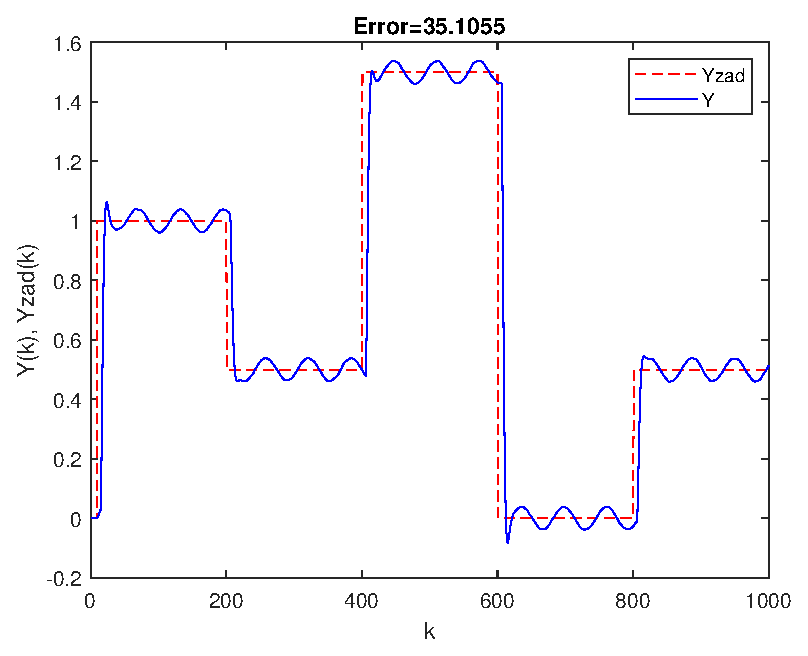
\includegraphics[scale=1]{Rys/szum-50}
	\label{fig:szum-50}
	\caption{Przebieg dla zakłócenia z parametrami $p=10$ oraz $a=0.1$ z szumem o mocy $-50 dBW$.}
\end{figure}
\begin{figure}[h!]
	\centering
	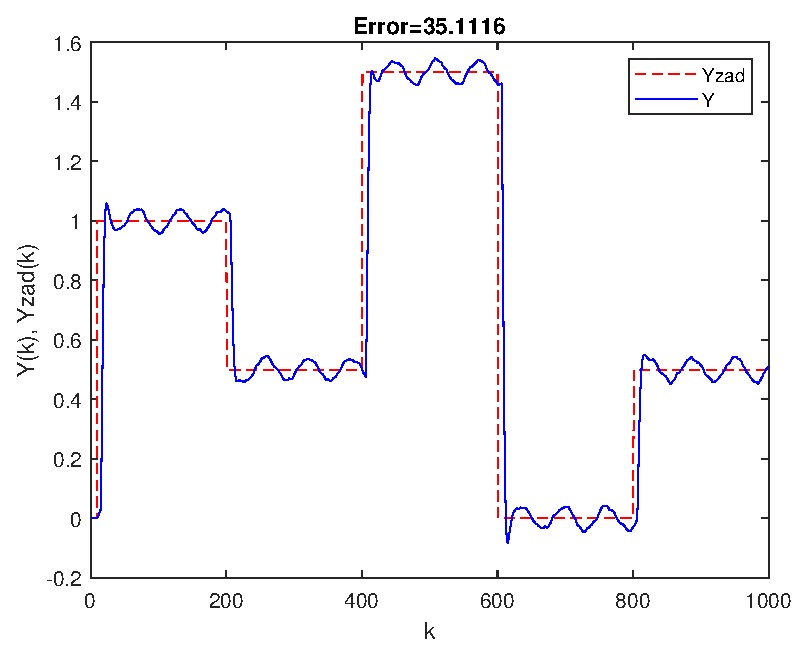
\includegraphics[scale=1]{Rys/szum-40}
	\label{fig:szum-40}
	\caption{Przebieg dla zakłócenia z parametrami $p=10$ oraz $a=0.1$ z szumem o mocy $-40 dBW$.}
\end{figure}
\begin{figure}[h!]
	\centering
	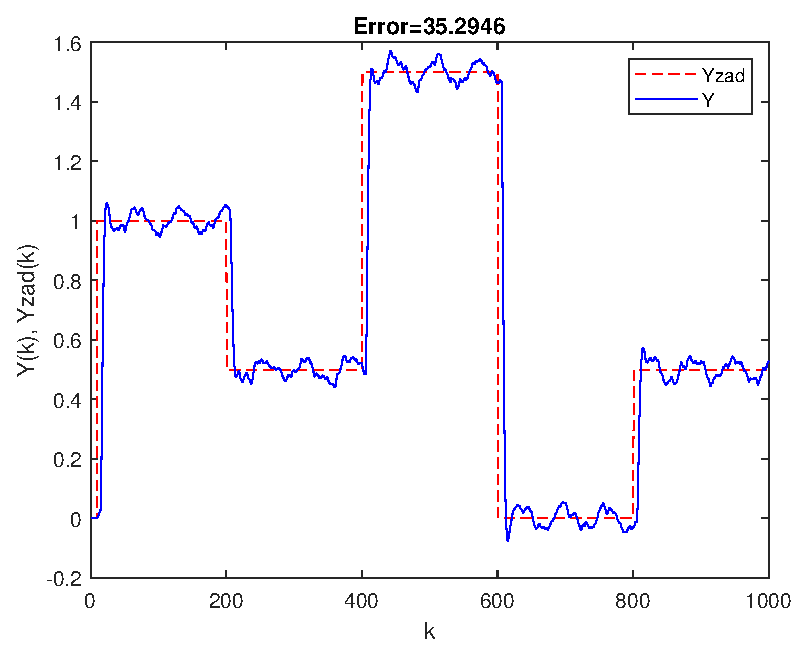
\includegraphics[scale=1]{Rys/szum-30}
	\label{fig:szum-30}
	\caption{Przebieg dla zakłócenia z parametrami $p=10$ oraz $a=0.1$ z szumem o mocy $-30 dBW$.}
\end{figure}
\begin{figure}[h!]
	\centering
	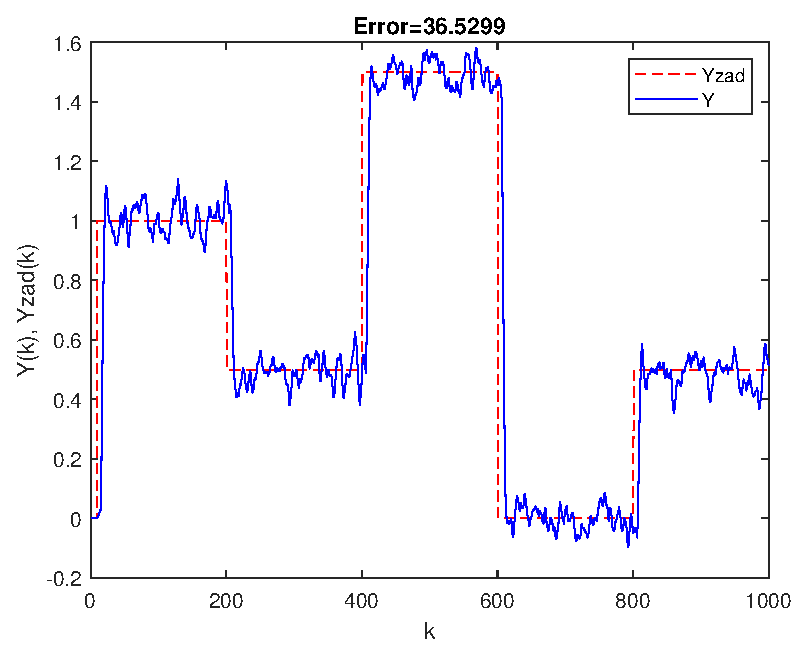
\includegraphics[scale=1]{Rys/szum-20}
	\label{fig:szum-20}
	\caption{Przebieg dla zakłócenia z parametrami $p=10$ oraz $a=0.1$ z szumem o mocy $-20 dBW$.}
\end{figure}
\begin{figure}[h!]
	\centering
	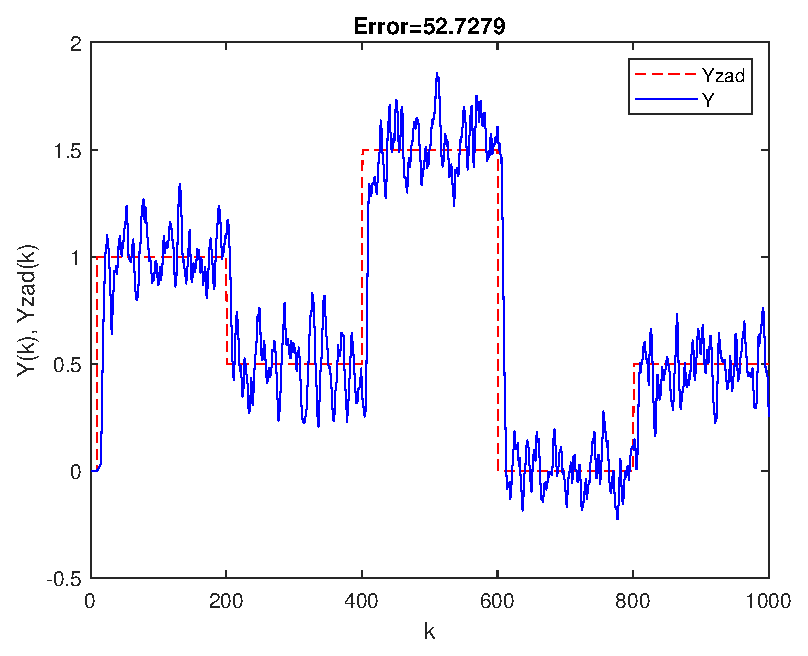
\includegraphics[scale=1]{Rys/szum-10}
	\label{fig:szum-10}
	\caption{Przebieg dla zakłócenia z parametrami $p=10$ oraz $a=0.1$ z szumem o mocy $-10 dBW$.}
\end{figure}
\begin{figure}[h!]
	\centering
	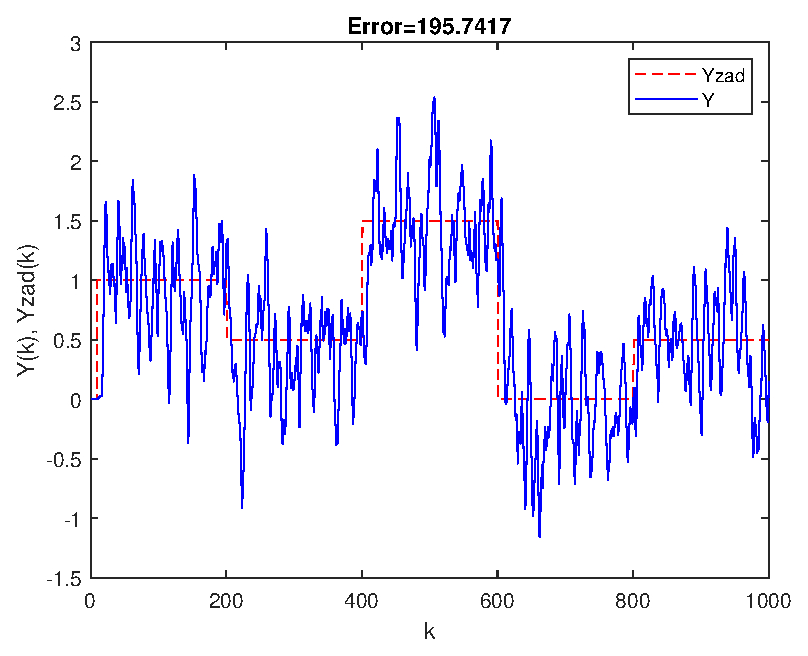
\includegraphics[scale=1]{Rys/szum0}
	\label{fig:szum0}
	\caption{Przebieg dla zakłócenia z parametrami $p=10$ oraz $a=0.1$ z szumem o mocy $0 dBW$.}
\end{figure}
\FloatBarrier
\subsection{Omówienie wyników}
Na powyższych wykresach można łatwo zaobserwować, że wraz z rosnącą mocą szumu pomiarowego jakość regulacji pogarszała się. Przy mocy o wartości $-10 dBW$ błąd regulacji okazał się być większy niż w przypadku gdy zakłócenie nie było brane pod uwagę. \\
Aby sprawdzić, jak zachowa się regulator przy tej samej mocy szumu, lecz przy większym zakłóceniu, wygenerowany został jeszcze jeden przebieg (rys. \ref{fig:szum1-10}). Można na nim zobaczyć, że jakość regulacji jest wciąż lepsza od regulatora bez pomiaru zakłócenia. \\
Należy zatem wywnioskować, że im większe jest zakłócenie, tym mniejszą rolę odgrywa szum pomiarowy, lecz w przypadku, gdy jest zbyt silny, lepiej stosować regulator bez uwzględniania zakłócenia.
\begin{figure}[h!]
	\centering
	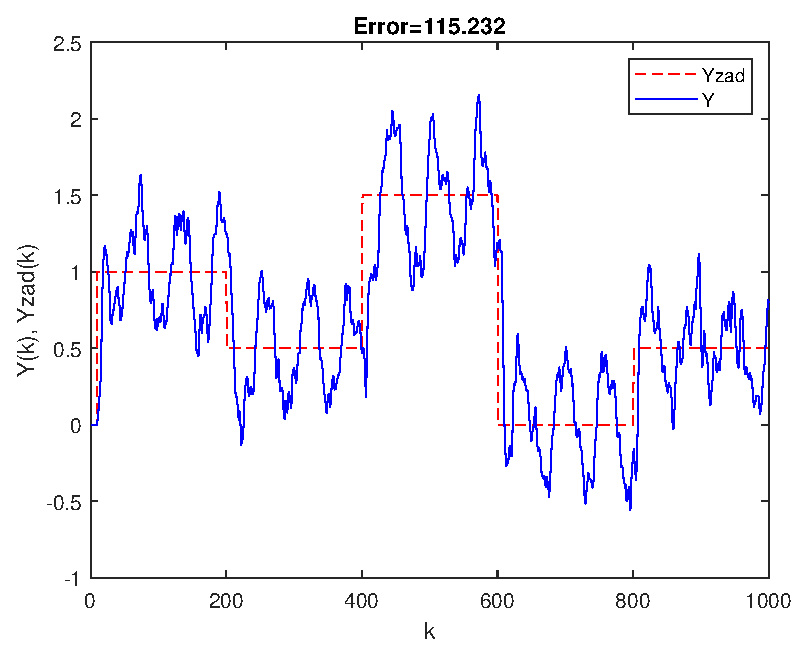
\includegraphics[scale=1]{Rys/szum1-10}
	\label{fig:szum1-10}
	\caption{Przebieg dla zakłócenia z parametrami $p=10$ oraz $a=1$ z szumem o mocy $-10 dBW$.}
\end{figure}